\chapter[Dinâmica dos sólidos computacional]{Dinâmica dos sólidos computacional} \label{capitulo:Cap4}

Assim como no caso da Mecânica dos Fluidos, um sólido é modelado como um corpo contínuo, com seu movimento governado por um conjunto de equações provenientes da lei da conservação da quantidade de movimento, lei da conservação da massa e lei da conservação de energia. Entretanto, diferentemente dos fluidos, os sólidos possuem resistência às solicitações tangenciais até que alcance seu limite resistente, e por isso, apresentam deslocamentos e deformações finitos. 

As variáveis de interesse na resolução do conjunto de equações que descrevem o comportamento do sólido são os deslocamentos, ou, posições atuais ao longo do tempo, dessa forma, uma descrição do tipo Lagrangiana é mais adequada para essas análises.

Nesse contexto, o comportamento estrutural pode ser classificado como linear ou não linear. No contexto do comportamento não linear, em geral, as não linearidades envolvidas podem ser de natureza geométrica, quando associadas à presença de grandes deslocamentos e rotações que não permitem aproximar a configuração atual pela inicial, ou de natureza física, quando resultam de modificações na relação constitutiva do material.

Para problemas de sólidos com comportamento elástico, quando houver a possibilidade de grandes deslocamentos, a não-linearidade geométrica deve ser contemplada no modelo matemático. Para isso, altera-se a forma de consideração do equilíbrio das forças no sólido. Enquanto que em uma modelagem geometricamente linear o equilíbrio é considerado na configuração inicial, que é muito próxima a configuração atual do corpo, em uma análise não-linear geométrica, o equilíbrio é considerado na configuração atual (ver, por exemplo \citeonline{Ogden:1984} e \citeonline{Coda:2018}).

Em muitos problemas da IFE, tal como o \textit{flutter}, grandes deslocamentos estão envolvidos. Desse modo, neste estudo utiliza-se uma formulação não-linear geométrica dinâmica de cascas baseada em uma descrição Lagrangiana Total para as análise dinâmica de estruturas. 

A formulação é baseada no método dos elementos finitos com abordagem posicional \cite{Coda:2003,Coda:2018}, onde as variáveis principais são as posições nodais. Escolheu-se trabalhar com elementos de cascas, uma vez que esses podem representar a maioria dos problemas estruturais tridimensionais. 

Considera-se a cinemática de Reissner-Mindlin, e adotam-se como parâmetros nodais as posições da superfície média, vetores generalizados, inicialmente unitários e perpendiculares à superfície média, e um termo de enriquecimento que permite considerar variação linear de deformação na direção da espessura, de acordo com \citeonline{SanchesC:2013}. Isso permite um mapeamento completo e flexível do elemento deformado. 

Neste capítulo, a formulação é apresentada a partir da descrição da cinemática e das condições de equilíbrio dos corpos deformáveis, com o objetivo de se deduzirem as equações globais de equilíbrio na descrição Lagrangiana, seguida pela introdução do modelo constitutivo de \textit{Saint-Venant–Kirchhoff}. Em seguida, aborda-se a formulação do método dos elementos finitos baseada em posição para ao elemento finito de casca adotado, a técnica de integração temporal e o algoritmo para solução, juntamente com um exemplo. Essa formulação foi desenvolvida, verificada e validada em diversos estudos \cite{Coda.., SanchesC:2013, SanchesC:2014, FernandesCS:2018} \textcolor{red}{citar trabalhos com casca dinâmica} e o código computacional já disponível no grupo de pesquisa foi aproveitado, de modo que não se preocupa com validação do código. 

\section{Cinemática dos corpos deformáveis}

Um sólido deformável quando sujeito à ações externas, sofre uma mudança de configuração. Nesta seção busca-se definir medidas pontuais para a deformação. Na \autoref{fig:solido_cinematica}, pode-se observar um sólido na sua configuração inicial $\Omega_{0}$, com coordenadas materiais descritas por $\lPosition$, e o mesmo sólido no instante atual, representado por $\Omega$, com coordenadas espaciais $\ePosition$. 

\begin{figure}[!htbp]
	\caption{Cinemática de um sólido deformável}
	\centering
	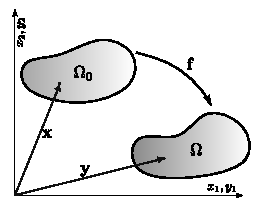
\includegraphics[scale=1.7]{Imagens/Cap4/sol_cinematica.pdf}	
	\label{fig:solido_cinematica}
	\legend{Fonte: Elaborada pela autora}
\end{figure}

A função mudança de configuração, denominada de $\fmap$, mapeia cada ponto da posição inicial para a atual, de modo que:

\begin{align}
	\ePosition = \fmap(\lPosition,t).
\end{align}

Uma medida de deformação Lagrangeana deve quantificar a mudança de forma em cada ponto do contínuo em relação ao estado inicial. Para o caso de grandes deslocamentos, assunto deste estudo, a medida de deformação deve ser independente de movimento de corpo rígido ou da escolha dos eixos de referência, ou seja, deve ser uma medida objetiva. A medida de deformação é descrita em termos do gradiente da função mudança de configuração, $\gradDeformation$, definido como:

\begin{align}
	\gradDeformation = \lGrad\left(\fmap\right) = \lGrad\ePosition.
\end{align}

\noindent onde o subscrito $\lPosition$ indica que o gradiente é tomado segundo as coordenadas da configuração material inicial.

A partir de $\gradDeformation$, é possível definir o tensor de deformações de Green-Lagrange (ver por exemplo \citeonline{Ogden:1984}), que é uma medida de deformação objetiva e normalizada dada por: 

\begin{align}
\greenStrain = \frac{1}{2}\left(\cauchyStretch - \unittensor\right),
\end{align}

\noindent onde $\cauchyStretch$ é um tensor simétrico denominado de tensor de alongamento à direita de Cauchy-Green dado por:

\begin{align}
\cauchyStretch = \gradDeformation^{t} \cdot \gradDeformation =  \gradDeformation \cdot \gradDeformation^{t}.
\end{align}

A partir do gradiente da função mudança de configuração pode-se estabelecer uma relação entre um vetor qualquer $\mathbf{u}$ definido na configuração inicial e seu equivalente na configuração atual $\mathbf{v}$ através da seguinte expressão:

\begin{align}
\mathbf{v} = \gradDeformation \cdot \mathbf{u} \label{eq:rel_vet}
\end{align}

Para a obtenção posteriormente das equações de equilíbrio em descrição Lagrangiana, faz-se necessário abordar as relações de mudança de volume e de área que ocorrem da configuração inicial para a atual. 

No estabelecimento de uma relação entre o volume inicial e final, definem-se dois volumes infinitesimais, um inicial $dV_{0}$ e um final $dV$, apresentados na \autoref{fig:solido_def_vol}. O volume infinitesimal inicial $dV_{0}$ pode ser calculado por:

\begin{align}
dV_{0} = (\mathbf{dx}_{1} \wedge \mathbf{dx}_{2}) \cdot \mathbf{dx}_{3} = \det{(\mathbf{dx_1},\mathbf{dx_2},\mathbf{dx_3})},
\end{align}

\noindent com $\mathbf{dx}_1,\mathbf{dx}_2$ e $\mathbf{dx}_3$ vetores materiais que definem o volume inicial. O volume atual pode ser expresso então, por:

\begin{align}
dV = (\mathbf{dy}_{1} \wedge \mathbf{dy}_{2}) \cdot \mathbf{dy}_{3} = \det{(\mathbf{dy_1},\mathbf{dy_2},\mathbf{dy_3})}, \label{eq:vol_atual}
\end{align}

\noindent  sendo $\mathbf{dy}_1,\mathbf{dy}_2$ e $\mathbf{dy}_3$ aos mesmos vetores $\mathbf{dx}_1,\mathbf{dx}_2$ e $\mathbf{dx}_3$ após a mudança de configuração.

Tendo em vista a expressão \ref{eq:rel_vet}, pode-se reescrever a \autoref{eq:vol_atual}, como:

\begin{align}
dV = \det{\left(\gradDeformation\right)} \cdot \det{(\mathbf{dx_1},\mathbf{dx_2},\mathbf{dx_3})}  = JdV_{0} \label {eq:vol_atual2},
\end{align}

\noindent na qual $J$ representa o determinante Jacobiano da função mudança de configuração.

\begin{figure}[!htbp]
	\caption{Mudança no volume}
	\centering
	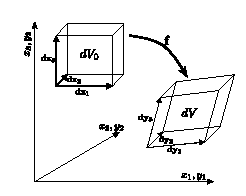
\includegraphics[scale=2.0]{Imagens/Cap4/sol_def_vol.pdf}	
	\label{fig:solido_def_vol}
	\legend{Fonte: Elaborada pela autora}
\end{figure}

Para escrever a relação entre uma área definida na configuração inicial e o seu valor na configuração atual, considera-se o cilindro apresentado na \autoref{fig:solido_def_area} em suas configurações inicial e atual. Sendo $\mathbf{N}$ e $\mathbf{n}$ os versores unitários normais às áreas inicial $dA_{0}$ e atual $dA$. Os volumes na configuração inicial ($dV_{0}$) e na configuração atual ($dV$) são calculados por:

\begin{align}
dV_{0} = \mathbf{u} \cdot \mathbf{dA}_{0} = \mathbf{u} \cdot \mathbf{N} dA_0 ,\\
dV = \mathbf{v} \cdot \mathbf{dA} = \mathbf{v} \cdot \mathbf{n} dA \label{eq:vol_func_area},
\end{align}

\noindent com $\mathbf{u}$ e $\mathbf{v}$ vetores não coplanares com as áreas inicial e atual, que ligam os centros da base e do topo do cilindro.

\begin{figure}[!htbp]
	\caption{Mudança de área}
	\centering
	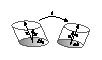
\includegraphics[scale=6.0,trim=0cm 0.2cm 0cm 0cm, clip=true]{Imagens/Cap4/sol_def_area.pdf}	
	\label{fig:solido_def_area}
	\legend{Fonte: Elaborada pela autora}
\end{figure}

Considerando a relação da \autoref{eq:rel_vet}, pode-se escrever o volume na configuração atual, $dV$, como:

\begin{align}
	dV = \mathbf{u} \cdot \gradDeformation^{t} \cdot \mathbf{n} dA = J dV_0 = J \mathbf{u} \cdot \mathbf{N} dA_0. \label{eq:dv}
\end{align}

Pré-multiplicando-se a \autoref{eq:dv} por ($(\gradDeformation^{t})^{-1}$) e considerando-se a arbitrariedade de $\mathbf{u}$, chega-se a conhecida fórmula de Nanson, descrita como:

\begin{align}
\mathbf{n}dA = J \gradDeformation^{-t} \cdot \mathbf{N} dA_{0}. \label{eq:Nanson}
\end{align}

aquiiiii.....

\section{Equilíbrio de corpos deformáveis} \label{capitulo:Cap3:EquilibrioCorposDeformaveis}

\subsection{Estado de tensão em um ponto}

Um corpo contínuo, ao ser submetido a ações externas, desenvolve forças internas de modo a garantir o equilíbrio dinâmico ou estático. A medida em cada ponto dessas forças internas é fundamental dentro da mecânica dos sólidos para a aplicação das leis da física às partículas do corpo.

Considerando um corpo qualquer, na configuração atual, sujeito a um conjunto equilibrado de forças externas, ao fazer-se a extração de um volume elementar infinitesimal, conforme pode ser observado na \autoref{fig:sol_equi}, surgem em suas faces, por ação e reação, uma distribuição de forças por unidade de superfície. Decompondo essas tensões em componentes cartesianas, obtém-se em cada face uma componente normal e duas componentes tangenciais de tensão. As componentes de tensão são designadas por $\sigma_{ij}$, com $i$ referindo-se ao plano de atuação e $j$ indicando a direção de atuação da tensão. Na \autoref{fig:sol_equi} podem ser observadas as componentes positivas de tensão em cada plano. No plano paralelo oposto, pela lei da ação e reação, as tensões possuem mesma intensidade, porém sentido contrário.

\begin{figure}[!htbp]
	\caption{Volume infinitesimal: componentes de tensão}
	\centering
	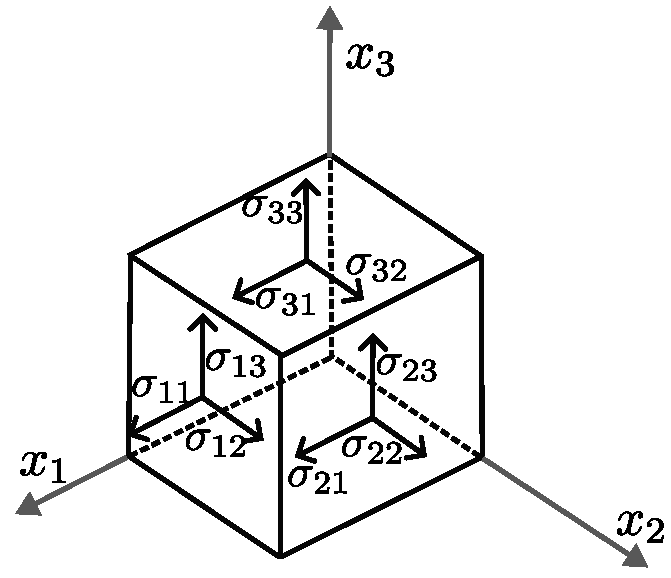
\includegraphics[scale=0.5,trim=0cm 0.0cm 0cm 0cm, clip=true]{Imagens/Cap4/sol_vol_equi.pdf}	
	\label{fig:sol_equi}
	\legend{Fonte: Elaborada pela autora}
\end{figure}

O tensor de tensões de Cauchy ($\cauchyStress$) contém todas as informações de tensão em um ponto e será representado como:

\begin{align}
\cauchyStress =
\begin{bmatrix}
	\sigma_{11} & \sigma_{12} & \sigma_{13} \\
	\sigma_{21} & \sigma_{22} & \sigma_{23} \\
	\sigma_{31} & \sigma_{32} & \sigma_{33}
\end{bmatrix}
.
\end{align}

Ao realizar-se o equilíbrio de momentos sobre um elemento infinitesimal, nota-se que $\cauchyStress$ é simétrico (Teorema de Cauchy), e pode ser reescrito como:

\begin{align}
	\cauchyStress =
	\begin{bmatrix}
		\sigma_{11} & \sigma_{12} & \sigma_{13} \\
		\sigma_{12} & \sigma_{22} & \sigma_{23} \\
		\sigma_{13} & \sigma_{23} & \sigma_{33}
	\end{bmatrix}
	.
\end{align}

Vale ressaltar que, a tensão de Cauchy é definida na configuração atual do contínuo, e por isso, trata-se de uma medida Euleriana de tensão.

Se extraíssemos do corpo contínuo um volume tetraédrico (\autoref{fig:sol_tetra}), no plano inclinado, cujo versor normal é $\mathbf{n}$, surge um vetor de tensões designado por $\mathbf{t}$. Considerando que a área do plano inclinado foi definida como $dA$, enquanto que as áreas correspondentes aos planos coordenados são suas projeções, pode-se calcular o equilíbrio do tetraedro em cada direção, chegando-se a seguinte expressão:

\begin{align}
	\mathbf{t} = \cauchyStress^{t} \cdot \mathbf{n} =  \cauchyStress \cdot \mathbf{n}.
\end{align}

\begin{figure}[!htbp]
	\caption{Tetraedro elementar}
	\centering
	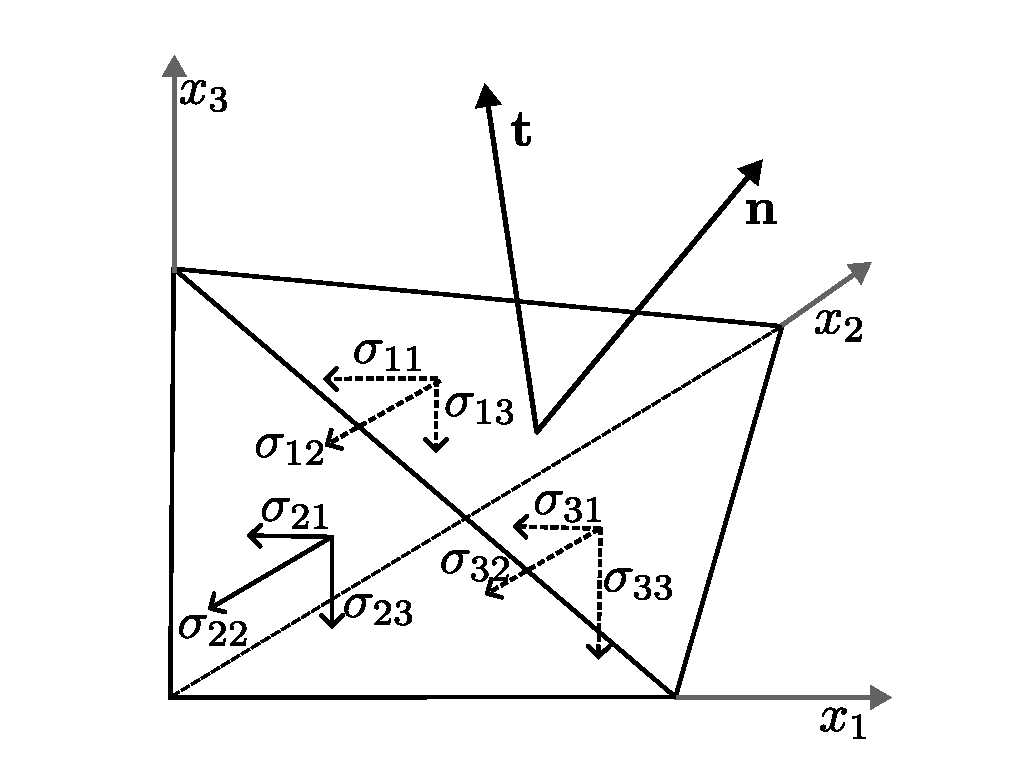
\includegraphics[scale=0.5,,trim=0cm 0.0cm 0cm 0cm, clip=true]{Imagens/Cap4/sol_tetra_equi.pdf}	
	\label{fig:sol_tetra}
	\legend{Fonte: Elaborada pela autora}
\end{figure}

Essa expressão é conhecida por fórmula de Cauchy. Considerando que o plano inclinado refere-se a superfície externa, essa equação pode ser utilizada para relacionar o estado de tensão em um ponto com as forças de superfície ($\mathbf{p}$), como:
 
\begin{align}
	\mathbf{p} = \cauchyStress^{t} \cdot \mathbf{n} =  \cauchyStress \cdot \mathbf{n}.
\end{align}


\subsection{Equilíbrio local Lagrangeano}

Para a obtenção das equações de equilíbrio local em descrição Lagrangeana, será utilizada como ponto de partida a equação de equilíbrio local Euleriana. Para isso, considere o sólido apresentado na \autoref{fig:sol_cargas}, o qual está submetido a forças de corpo, $\ebodyLoad$, e a forças de superfície, $\tractionLoad$. Extraindo-se um elemento infinitesimal deste corpo que sofreu mudança de configuração, e aplicando-se a segunda Lei de Newton, o  equilíbrio local pode ser descrito:

\begin{align}
	\gradient \cdot \stressTensor^{t} + \ebodyLoad = \rho  \solidAccel, \label{eq:equi_local_euleriano}
\end{align}

\noindent ou ainda, em notação indicial:

\begin{align}
	\sigma_{ji,j} + b_i  = \rho  \ddot{y_i},
\end{align}

\noindent com $\rho$ representando a massa específica do material que compõe o sólido e $\solidAccel$ é a derivada material da velocidade do ponto material (aceleração do corpo).

\begin{figure}[!htbp]
	\caption{Sólido sob carregamento externo}
	\centering
	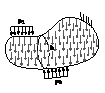
\includegraphics[scale=4,trim=0cm 0.0cm 0cm 0cm, clip=true]{Imagens/Cap4/sol_cargas.pdf}	
	\label{fig:sol_cargas}
	\legend{Fonte: Elaborada pela autora}
\end{figure}

Ao integrar-se a \autoref{eq:equi_local_euleriano} no volume do sólido e utilizar-se o Teorema da Divergência chega-se a:

\begin{align}
	\int_{A} {\stressTensor}^{t} \cdot \mathbf{n} dA + \int_{V} \ebodyLoad dV = \int_{V} \rho  \solidAccel dV \label{eq:eq_global_euleriano}
\end{align}

\noindent ou, ainda:

\begin{align}
	\int_{A} \mathbf{p} dA + \int_{V} \ebodyLoad dV = \int_{V} \rho  \solidAccel dV 
\end{align}

Considerando as relações de mudança de área e volume, apresentadas nas equações \autoref{eq:vol_atual2} e \autoref{eq:Nanson}, e que da equação da conservação da massa ($M$) tem-se que:

\begin{align}
	M = \int_{V_{0}} \rho_{0}dV_{0} = \int_{V(t)} \rho(t)dV, \label{eq:conser_massa}
\end{align}

\noindent escreve-se a equação global de equilíbrio Lagrangeana, a partir da \autoref{eq:eq_global_euleriano} como:

\begin{align}
	\int_{A_0} \mathbf{P}^t \cdot \mathbf{N} dA_0 + \int_{V_0} \bodyLoad dV_0 = \int_{V_0} \rho_0  \solidAccel dV_0, \label{eq:equi_global_lagrangeano}
\end{align}

\noindent na qual o primeiro tensor de tensões transposto de Piola-Kirchhoff ($\mathbf{P}^t$), não simétrico, é definido como $\mathbf{P}^t = J \stressTensor^t \cdot \mathbf{B}$, e o subíndice $0$, refere-se a variável no instante inicial.

Ao aplicar-se o Teorema da Divergência a \autoref{eq:equi_global_lagrangeano} e da consideração da arbitrariedade do volume, chega-se a versão local da equação de equilíbrio Lagrangeano, expressa por:

\begin{align}
	\lGrad \cdot \mathbf{P}^t +  \bodyLoad = \rho_0  \solidAccel. \label{eq:equi_local_lagrangeano}
\end{align}


\subsection{Princípio de Estacionariedade de energia}

No estudo do equilíbrio de corpos deformáveis a análise da energia mecânica é um assunto de grande importância. A energia mecânica é formada basicamente por três parcelas: energia potencial das forças externas ($\extEnergy$), energia de deformação ($\intEnergy$) e energia cinética ($\kinEnergy$). A energia total mecânica ($\totalEnergy$) é um funcional obtido pela soma dessas três parcelas, sendo escrita da seguinte maneira:

\begin{align}
	\totalEnergy = \extEnergy + \kinEnergy + \intEnergy.
\end{align}

O princípio da estacionariedade da energia define que um corpo quando em equilíbrio apresenta a primeira variação do funcional de energia mecânica nula, sendo o equilíbrio estável quando a posição de equilíbrio representa um mínimo local para a energia mecânica total. Este princípio, para uma descrição das equações de equilíbrio em posições, pode ser expresso matematicamente da seguinte forma:

\begin{align}
	\delta\totalEnergy = \frac{\partial{\totalEnergy}}{\partial{\ePosition}} \cdot \delta\ePosition = \mathbf{0}, \label{eq:princ_esta}
\end{align}

\noindent ou, dada a arbitrariedade de $\delta\ePosition$, como: 

\begin{align}
	\delta\totalEnergy = \delta\extEnergy + \delta\kinEnergy + \delta\intEnergy.
\end{align}

Um incremento de energia mecânica específica (energia mecânica por unidade de volume) pode ser obtido pelo produto escalar da \autoref{eq:equi_local_lagrangeano} por um incremento de posição $\delta\ePosition$, e, integrando-se sobre o domínio inicial, têm-se:

\begin{align}
	\delta\totalEnergy = \int_{V_0} \left(\rho_0 \solidAccel - \lGrad \cdot \mathbf{P}^t -  \ebodyLoad_0 \right) \cdot  \delta\ePosition dV_0 = 0 \label{eq:equi_local_forma_frac}
\end{align}

Ao integrar-se por partes o segundo termo da \autoref{eq:equi_local_forma_frac} e utilizar-se o Teorema da Divergência, chega-se a seguinte expressão:

\begin{align}
	\delta\totalEnergy = \int_{V_0} \rho_0 \solidAccel \cdot \delta\ePosition dV_0 - \int_{A_0} \mathbf{P}^t \cdot \mathbf{N} \cdot  \delta\ePosition dA_0  + \int_{V_0} \mathbf{P}^t : \lGrad(\delta\ePosition) dV_0 - \int_{V_0} \mathbf{b_0} \cdot \delta \ePosition dV_0 = 0 \label{eq:equi_local_forma_frac2}
\end{align}

A \autoref {eq:equi_local_forma_frac2} pode ainda ser reformulada, considerando que $\lGrad (\delta\ePosition) = \delta \gradDeformation$ e que $\mathbf{P}^t \cdot \mathbf{N}$ representa as forças de superfície na configuração inicial ($\ltractionLoad$) como:

\begin{align}
\delta\totalEnergy = \int_{V_{0}} \rho_{0} \solidAccel \cdot \delta\ePosition dV_{0} - \int_{A_{0}} \ltractionLoad \cdot \delta\ePosition dA_{0} + \int_{V_{0}} \mathbf{P}^{t} : \delta\gradDeformation dV_{0} - \int_{V_{0}}  \bodyLoad \cdot \delta\ePosition dV_{0} = 0. \label{eq:equi_local_forma_frac3}
\end{align}

Conforme relatou-se, o tensor de Piola-Kirchhoff de primeira espécie não é necessariamente simétrico, desta forma, torna-se mais conveniente adotar uma medida de tensão que resulte em um tensor simétrico. Com essa finalidade, adota-se um tensor $\piolaStress$, de forma que:

\begin{align}
\mathbf{P} = \piolaStress^{t} \cdot \gradDeformation^{t}, \label{eq:piola-kircchoff}
\end{align}

\noindent com $\piolaStress$ conhecido como tensor de Piola-Kirchhoff de segunda espécie. 

Utilizando-se a relação apresentada na \autoref{eq:piola-kircchoff} na \autoref{eq:equi_local_forma_frac3}, chega-se a:

\begin{align}
\delta\totalEnergy = \int_{V_{0}} \rho_{0} \solidAccel \cdot \delta\ePosition dV_{0} - \int_{A_{0}} \ltractionLoad \cdot \delta\ePosition dA_{0} +  \int_{V_{0}} \piolaStress : \delta\greenStrain dV_{0} - \int_{V_{0}}  \bodyLoad \cdot \delta\ePosition dV_{0} = 0.
\label{eq:equi_local_forma_final0}
\end{align}

A \autoref{eq:equi_local_forma_final0}, será adicionada ainda uma parcela referente a possibilidade de carregamentos pontuais, sendo expressa então, por:

\begin{align}
	\delta\totalEnergy = \int_{V_{0}} \rho_{0} \solidAccel \cdot \delta\ePosition dV_{0} - \int_{A_{0}} \ltractionLoad \cdot \delta\ePosition dA_{0} +  \int_{V_{0}} \piolaStress : \delta\greenStrain dV_{0} - \int_{V_{0}}  \bodyLoad \cdot \delta\ePosition dV_{0} - \mathbf{F} \cdot \delta\ePosition = 0.
	\label{eq:equi_local_forma_final}
\end{align}

Partindo-se da \autoref{eq:equi_local_forma_final}, encontra-se a relação entre suas componentes e as parcelas de energia mecânica, dessa forma, têm-se:

\begin{align}
	 \delta\extEnergy = - \int_{A_{0}} \ltractionLoad \cdot \delta\ePosition dA_{0} - \int_{V_{0}}  \bodyLoad \cdot \delta\ePosition dV_{0} - \mathbf{F} \cdot \delta\ePosition,
\end{align}

\begin{align}
	\delta\kinEnergy = \int_{V_{0}} \rho_{0} \solidAccel \cdot \delta\ePosition dV_{0},
\end{align}

\begin{align}
	 \delta\intEnergy = \int_{V_{0}} \piolaStress : \delta\greenStrain dV_{0}.
\end{align}

\subsection{Modelo constitutivo de Saint-Venant-Kirchhoff}

A lei constitutiva hiperelástica de Saint-Venant-Kirchhoff estabelece uma relação linear entre o tensor das tensões de Piola Kirchhoff de segunda espécie e o tensor de deformação de Green, e pode ser escrita pela expressão generalizada da energia de deformação por:

\begin{align}
u_{e} = \frac{1}{2} \greenStrain : \constitutiveTensor : \greenStrain,
\end{align}

\noindent ou, em notação indicial:

\begin{align}
u_{e} = \frac{1}{2} E_{kl} C_{klij} E_{ij}
\end{align}

\noindent com $\constitutiveTensor$ representando o tensor constitutivo elástico isotrópico, que é um tensor de quarta ordem definido como:

\begin{gather}
\constitutiveTensor_{ijkl}=\left(\bulkModulus - \frac{2}{3}\shearModulus \right)\delta_{ij}\delta_{kl} + \shearModulus(\delta_{ik}\delta_{jl}+\delta_{il}\delta_{jk}),
\end{gather}

\noindent sendo $\delta_{ij}$ o delta de Kronocker, $\bulkModulus$ e $\shearModulus$ os módulos volumétrico e de cisalhamento respectivamente, os quais são calculados através das seguintes relações:

\begin{gather}
\bulkModulus=\lameParameter+\frac{2}{3}\shearModulus,\\
\shearModulus=\frac{\elasticModulus}{2(1+\poisonsRatio)},\\
\lameParameter=\frac{\poisonsRatio \elasticModulus}{(1+\poisonsRatio)(1-2\poisonsRatio)},
\end{gather}

\noindent com $\elasticModulus$ sendo o módulo de elasticidade longitudinal e $\poisonsRatio$ o coeficiente de Poisson. Ressalta-se que essa lei constitutiva aqui utilizada é adequada para grandes deslocamentos, entretanto, a mesma é adequada somente para deformações pequenas a moderadas.

\section{Método dos Elementos Finitos Posicional}

Conforme discutido na \autoref{capitulo:Cap2:FormaFraca:ElementosFinitos}, o método dos elementos finitos baseia-se na substituição do contínuo por um conjunto finito de subdomínios, denominados elementos finitos. Em cada um desses elementos, as variáveis de interesse — incluindo a própria geometria — são aproximadas, de modo que o problema contínuo é convertido em um problema discreto, caracterizado por um número finito de incógnitas.

Nesta subseção será apresentado o desenvolvimento da formulação posicional do Método dos Elementos Finitos aplicada a cinemática de cascas.

\subsection{Elemento finito de Casca} \label{capitulo:Cap4:Mef:Casca}

A formulação não-linear geométrica de casca posicional foi desenvolvida por \citeonline{CodaP:2007}, e consistia inicialmente em 6 graus de liberdade por nó, sendo 3 referentes à posições e 3 referentes às componentes do vetor generalizado. Em \citeonline{CodaP:2008} incluí-se a formulação um sétimo parâmetro, que considera a taxa de variação linear da espessura, para lidar com o fenômeno de travamento volumétrico. Essa última cinemática será utilizada nesse trabalho.

As cascas são sólidos que possuem uma de suas dimensões muito menor do que as outras, assim o mapeamento da configuração do sólido pode ser facilitado tomando-se a superfície média como referência. Os mapeamentos das configurações inicial e atual dos pontos da superfície média, conforme pode ser observado na \autoref{fig:casca:map_super_media}, são definidos respectivamente como:

\begin{align}
\fmap^{mh}_{0}(\xi_{1},\xi_{2}) = \lPosition^{mh}(\xi_{1},\xi_{2}) = N_{l} (\xi_{1},\xi_{2}) \lPosition_{l}^{mh}\label{eq:casca_Lposition_m}\\
\fmap^{mh}_{1}(\xi_{1},\xi_{2}) = \ePosition^{mh}(\xi_{1},\xi_{2}) = N_{l} (\xi_{1},\xi_{2}) \ePosition_{l}^{mh}, \label{eq:casca_Eposition_m}
\end{align}

\noindent com $\lPosition_{l}^{mh}$ e $\ePosition_{l}^{mh}$ representando os vetores dos parâmetros de posição inicial e atual da linha média respectivos ao nó $l$, e, $N_{l} (\xi_{1},\xi_{2})$ é o valor da função de forma do nó $l$ calculado no ponto de coordenadas paramétricas $(\xi_{1},\xi_{2})$.

\begin{figure}[!htbp]
	\caption{Mapeamento da superfície média da casca}
	\centering
	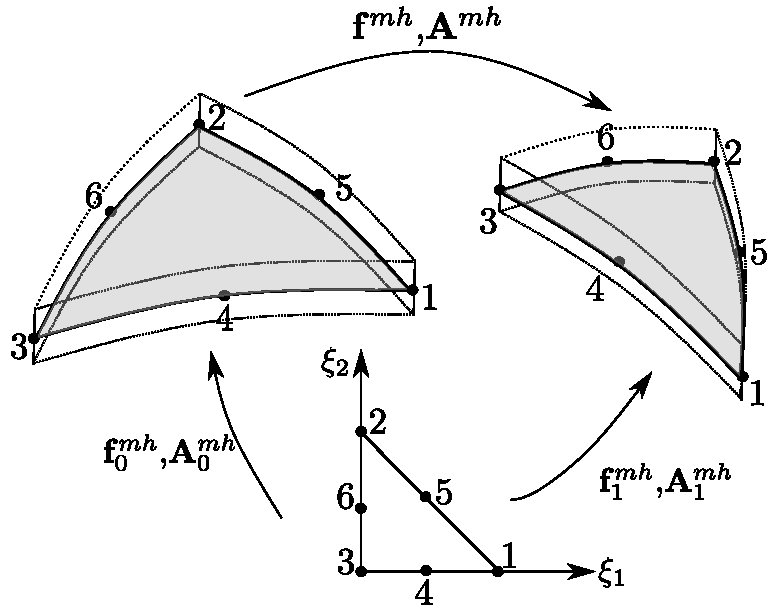
\includegraphics[scale=0.8,trim=0cm 0.0cm 0cm 0cm, clip=true]{Imagens/Cap4/casca_super_media.pdf}	
	\label{fig:casca:map_super_media}
	\legend{Fonte: Elaborada pela autora}
\end{figure}

Para completar a cinemática da casca, os demais pontos são mapeados por meio da soma da posição de um ponto na superfície média com um vetor generalizado $\mathbf{g}^{h}_{0}$ ou $\mathbf{g}^{h}_{0}$ nas configurações inicial e atual, respectivamente.  $\mathbf{g}^{h}_{0}$ é normal a linha de referência na configuração inicial, conforme pode ser observado na \autoref{fig:casca_vetores_generalizados}. Desta forma, o mapeamento completo fica definido por:

\begin{align}
\fmap^{h}_{0}(\xi_{1},\xi_{2},\xi_{3}) = \lPosition^{h}(\xi_{1},\xi_{2},\xi_{3}) = \fmap^{mh}_{0}(\xi_{1},\xi_{2}) + \mathbf{g}^{h}_{0} (\xi_{1},\xi_{2}, \xi_{3}) \label{eq:fmap0}\\
\fmap^{h}_{1}(\xi_{1},\xi_{2},\xi_{3}) = \ePosition^{h}(\xi_{1},\xi_{2},\xi_{3}) = \fmap^{mh}_{1}(\xi_{1},\xi_{2}) + \mathbf{g}^{h}_{1} (\xi_{1},\xi_{2}, \xi_{3})  \label{eq:fmap1}
\end{align}

\noindent em que $\xi_3$ é a coordenada adimensional na espessura da casca variando de -1 a 1.

\begin{figure}[!htbp]
	\caption{Vetores generalizados}
	\centering
	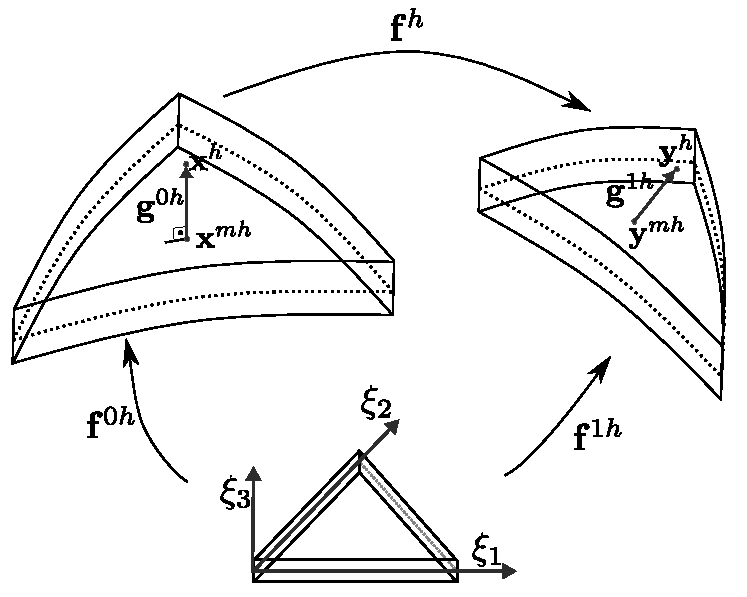
\includegraphics[scale=0.8,trim=0cm 0.0cm 0cm 0cm, clip=true]{Imagens/Cap4/casca_vetores_generalizados.pdf}	
	\label{fig:casca_vetores_generalizados}
	\legend{Fonte: Elaborada pela autora}
\end{figure}

Os vetores generalizados $\mathbf{g}^{h}_{0}$ e $\mathbf{g}^{h}_{1}$ representados na discretização por elementos finitos ficam expressos por:

\begin{align}
\mathbf{g}^{h}_{0} (\xi_{1},\xi_{2}, \xi_{3}) = \frac{h_{0}}{2}\xi_{3} N_{l}\left(\xi_{1},\xi_{2}\right) \cdot  (\mathbf{e}_x)_l, \\
\mathbf{g}^{h}_{1} (\xi_{1},\xi_{2}, \xi_{3}) = \frac{h_{0}}{2}\left[\xi_{3} + \eta_l N_l\left(\xi_{1},\xi_{2}\right)\xi_{3}^2\right]N_{l}\left(\xi_{1},\xi_{2}\right) \cdot (\mathbf{e}_y)_l,
\end{align}

\noindent com $h_{0}$ representando a espessura média inicial do elemento de casca, $(\mathbf{e}_x)_l$ é o l-ésimo valor nodal do vetor unitário normal à linha de referência inicial, $(\mathbf{e}_y)_l$ o l-ésimo valor nodal do vetor generalizado na configuração atual e $\eta_l$ é o l-ésimo valor nodal da chamada de taxa linear de variação da espessura.

Finalmente, defini-se a função mudança de configura, através da seguinte relação:

\begin{align}
	\fmap^{h} = \fmap^{h}_{1} \circ  (\fmap^{h}_{0})^{-1} \label{eq:eq_mud_conf}.
\end{align}

De forma análoga pode-se representar o gradiente de  $\fmap^{h}$ como:

\begin{align}
\gradDeformation^{h} = \gradDeformation^{h}_{1} \cdot \left(\gradDeformation^{h}_{0}\right)^{-1} \label{eq:gradDeformation},
\end{align}

\noindent em que $\gradDeformation^{h} = \lGrad \fmap^{h}$, $\gradDeformation^{h}_{0} = \frac{\partial  \fmap^{h}_{0}} {\partial \adimensionalcoordinates}$ e  $\gradDeformation^{h}_{1} =  \frac{\partial  \fmap^{h}_{1}} {\partial \adimensionalcoordinates}$.

Assim, o alongamento à direta de Cauchy-Green e a deformação de Green podem ser escritos em função de $\gradDeformation^{h}_{0}$ e $\gradDeformation^{h}_{1}$, como:

\begin{align}
	\cauchyStretch = \gradDeformation^{t} \cdot \gradDeformation = \left(\gradDeformation^{h}_{1} \cdot (\gradDeformation^{h}_{0})^{-1}\right)^{t} \cdot \left(\gradDeformation^{h}_{1} \cdot (\gradDeformation^{h}_{0})^{-1}\right),
\end{align}

\begin{align}
	\greenStrain = \frac{1}{2}\left(\cauchyStretch - \unittensor\right) = \frac{1}{2}\left(\left(\gradDeformation^{h}_{1} \cdot (\gradDeformation^{h}_{0})^{-1}\right)^{t} \cdot \left(\gradDeformation^{h}_{1} \cdot (\gradDeformation^{h}_{0})^{-1}\right) - \unittensor\right).
\end{align}

Neste trabalho, aplicou-se nas discretizações um elemento triangular quadrático com 6 nós.

Partindo do mapeamento apresentado é possível escrever o funcional de energia mecânica em função dos parâmetros nodais apresentados, e ao discretizar-se as equações no tempo, a solução do problema consiste encontrar os parâmetros nodais que satisfaçam:

\begin{align}
	\frac{\partial\totalEnergy^{h}}{\partial \ePosition_{l}^{mh}} = \frac{\partial\totalEnergy^{h}}{\partial (\mathbf{e}_y)_l} = \frac{\partial\totalEnergy^{h}}{\partial \eta_l} = \mathbf{0}.
\end{align}

\subsection{Integração Temporal e solução do problema não-linear}

Para a resolução do problema não-linear, vamos reescrever o princípio da estacionariedade em função da variável $\SolidPos$, que consiste em um vetor que contém todos os parâmetros nodais da estrutura (posições, vetores generalizados e taxa de variação linear da espessura) da seguinte forma:

\begin{align}
	\frac{\partial\totalEnergy}{\partial\SolidPos} = \frac{\partial\extEnergy}{\partial \SolidPos} + \frac{\partial\kinEnergy}{\partial \SolidPos} + \frac{\partial\intEnergy}{\partial \SolidPos} = \mathbf{0},
\end{align}

\noindent ou ainda,

\begin{align}
	- \concLoad^{ext}(t) + \solidMass\SolidAccel_{}+ \concLoad^{int}(\SolidPos) + \solidDamping\SolidVel_{} = \mathbf{0}, \label{eq:equi_forma_matricial}
\end{align}

\noindent na qual $ \concLoad^{int}(\SolidPos)$ representa as forças internas provenientes da variação da energia potencial interna, $\solidMass$ é a conhecida como matriz de massa proveniente da variação da energia cinética e $\mathbf{F}^{ext}$ representam as forças externas na estrutura fruto da variação da energia potencial das forças externas. O termo $\solidDamping$ representa uma matriz de amortecimento proporcional a massa, e $\SolidVel_{}$ a velocidade nodal.

Nesse trabalho, para a discretização temporal das equações, será utilizado o integrador de Newmark, visto que o mesmo demonstrou estabilidade e eficácia na vasta gama de trabalhos envolvendo o MEF posicional com sua aplicação (\cite{CodaG:2004,CodaP:2010,CarrazedoC:2010,CodaP:2011,SanchesC:2016}).
  
A integração temporal das equações inicia-se com a discretização do tempo de maneira que:

\begin{align}
	t_{n+1} = t_{n} + \Delta t, \label{eq:disc_tempo}
\end{align}

\noindent na qual $t_{n+1}$ representa o tempo no instante atual, $t_{n}$ o instante de tempo anterior e  $\Delta t$ o intervalo de tempo utilizado na discretização. Utilizando as aproximações de Newmark, posição, velocidade e aceleração nos tempos $n+1$ e $n$ são relacionados por:

\begin{gather}
	\SolidPos_{n+1}=\SolidPos_{n} + \timeStep \SolidVel_{n}+\left(\frac{1}{2}-\beta\right) \timeStep^2 \SolidAccel_{n}+ \beta \timeStep^2 \SolidAccel_{n+1},\label{eq:newmark1}\\
	\SolidVel_{n+1} = \SolidVel_{n}+(1-\gamma)\timeStep \SolidAccel_{n}+\gamma \timeStep \SolidAccel_{n+1},\label{eq:newmark2}
\end{gather}

\noindent em que $\beta$ e $\gamma$ são parâmetros dependentes do comportamento assumido para a aceleração. Para um aceleração constante adotada-se nesse trabalho $\gamma=\sfrac{1}{2}$ e $\beta=\sfrac{1}{4}$.

Partindo das equações \autoref{eq:newmark1} e \autoref{eq:newmark2} é possível escrever a aceleração e a velocidade atual em função das posições no instante $n+1$, as incógnitas do problema, e das demais variáveis do passo anterior:

\begin{align}
	\SolidAccel_{n+1} = \frac{1}{\beta \Delta_{t}^2}\SolidPos_{n+1} - \mathbf{Q}(t_n), \label{eq:accel_newmark}
\end{align}

\begin{align}
	\SolidVel_{n+1} = \frac{\gamma}{\beta \Delta_{t}}\SolidPos_{n+1} + \mathbf{R}(t_n) - \gamma \Delta_{t} \mathbf{Q}(t_n), \label{eq:vel_newmark}
\end{align}

\noindent em que:

\begin{gather}
	\mathbf{Q}(t_n) = \frac{\SolidPos_n}{\beta \timeStep^2} + \frac{\SolidVel_n}{\beta \timeStep} + \left(\frac{1}{2\beta} -1 \right)\SolidAccel_n,\label{eq:Qn}\\
	\mathbf{R}(t_n) = \SolidVel_n+\timeStep(1-\gamma)\SolidAccel_n.\label{eq:Rn}
\end{gather}

Utilizando as equações \autoref{eq:accel_newmark} e \autoref{eq:vel_newmark} na equação do equilíbrio em forma matricial (\autoref{eq:equi_forma_matricial}), tem-se para o instante $t_{n+1}$ a seguinte relação:

\begin{gather}
	\concLoad^{int}_{n+1}- \concLoad^{ext}_{n+1} + \frac{\solidMass}{\beta \timeStep^2} \SolidPos_{n+1}-\solidMass \mathbf{Q}_n+ \solidDamping\mathbf{R}_n + \frac{\gamma \solidDamping}{\beta \timeStep}\SolidPos_{n+1} - \gamma\timeStep \solidDamping\mathbf{Q}_n = \mathbf{0},
	\label{eq:equilibrio_tn+1}
\end{gather}
  
Pode-se escrever ainda o problema não linear definido pela \autoref{eq:equilibrio_tn+1} em função do resíduo da equação governante
discretizada no espaço e no tempo, como:

\begin{gather}
\NNSS\left(\SolidPos_{n+1}\right) = \concLoad^{int}_{n+1}- \concLoad^{ext}_{n+1} + \frac{\solidMass}{\beta \timeStep^2} \SolidPos_{n+1}-\solidMass \mathbf{Q}_n+ \solidDamping\mathbf{R}_n + \frac{\gamma \solidDamping}{\beta \timeStep}\SolidPos_{n+1} - \gamma\timeStep \solidDamping\mathbf{Q}_n= \mathbf{0}.
\label{eq:residuo_equilibrio_newmark}
\end{gather}

O problema não linear da \autoref{eq:residuo_equilibrio_newmark} é resolvido por meio do método iterativo de Newton-Raphson. Para isso, realiza-se uma expansão em série de Taylor de primeira ordem:

\begin{gather}
\NNSS\left(\SolidPos_{n+1}^{i+1}\right) \approx \NNSS\left(\SolidPos_{n+1}^{i}\right) + \Delta\NNSS\left(\SolidPos_{n+1}^{i}\right)\Delta\SolidPos_{n+1}^{i} 
\end{gather}

\noindent em que $i$ indica o índice da iteração atual. Na primeira iteração para o cálculo de $\SolidPos_{n+1}$ utiliza-se como predição da iteração anterior os valores das variáveis no passo de tempo $n$. O método de Newton-Raphson consiste em resolver o seguinte sistema:

\begin{gather}
\Delta\NNSS\left(\SolidPos_{n+1}^{i}\right)\Delta\SolidPos_{n+1}^{i} = -\NNSS\left(\SolidPos_{n+1}^{i}\right) \label{eq:NR}
\end{gather}

\noindent com:

\begin{gather}
\Delta\NNSS\left(\SolidPos_{n+1}^{i}\right) = \frac{\partial^{2}\totalEnergy}{\partial\SolidPos^{2}} = \frac{\partial^{2}\intEnergy}{\partial \SolidPos^{2}} + \frac{\solidMass}{\beta \timeStep^2} + \frac{\gamma \solidDamping}{\beta \timeStep}.
\end{gather}

A cada iteração de Newton-Raphson atualiza-se a posição, a aceleração e a velocidade de acordo com as seguintes equações:

\begin{gather}
\SolidPos_{n+1}^{i+1} = \SolidPos_{n+1}^{i} + \Delta\SolidPos_{n+1}^{i} \label{UD1}\\
\SolidAccel_{n+1}^{i+1} = \frac{\SolidPos_{n+1}^{i+1}}{\beta \timeStep^2} + \mathbf{Q}_n  \label{UD2} \\
\SolidVel_{n+1}^{i+1} = \frac{\gamma \SolidPos_{n+1}^{i+1}}{\beta \timeStep} + \mathbf{R}_n - \gamma\Delta t \mathbf{Q}_n  \label{UD3}
\end{gather}

Para mais detalhes a cerca da obtenção das matrizes e vetores do método, recomenda-se a consulta de \citeonline{Coda:2018}.

\subsection{Implementação Computacional}

Emprega-se nesse estudo, o programa computacional de análise não-linear dinâmica de sólidos cedido pelo aluno de doutorado Rosicley Junior Rodrigues Rosa, que faz parte do grupo de pesquisa da presente autora (GRUMEC) no Programa de Pós-Graduação em Engenharia de Estruturas da Escola de Engenharia de São Carlos - USP. O referido autor começou a desenvolver o código em seu trabalho de dissertação \cite{Rosa:2021}, o qual continua em desenvolvimento atualmente em sua tese de doutorado.

O código foi desenvolvido em linguagem C++ utilizando paralelização em protocolo MPI. Ressalta-se que a implementação conta com uma estratégia de acoplamento entre elementos não coplanares, que pode ser vista em \citeonline{Coda:2018}. O algoritmo que descreve a implementação computacional pode ser visualizado em Alg. \ref{alg:algoritmo_solid}. No algoritmo a variável $\mathbf{X}$ consiste em um vetor das variáveis nodais na configuração inicial.

\begin{algorithm}
	\caption{Algoritmo para problemas não-lineares dinâmicos utilizando MEF posicional}
	\label{alg:algoritmo_solid}
	\begin{algorithmic}[1]
		\State Adota-se $\SolidPos = \mathbf{X}$;
		\For {o passo de tempo $0$ até $\totalTime$} 
		\State $i=0$;
		\State Predição da solução: 
		\begin{align}
		\SolidPos_{n+1}^{0} = \SolidPos_{n},\\
		\SolidVel_{n+1}^{0} = \SolidVel_{n},\\
		\SolidAccel_{n+1}^{0} = \SolidAccel_{n};
		\end{align}
		\State Calcula-se  nível de força aplicado $\concLoad^{ext}_{n+1}(t_{n+1})$ e/ou as posições prescritas $\SolidPos_{n+1}$;
		\State Calculam-se os valores de $\mathbf{Q}_n$ (\autoref{eq:Qn}) e $\mathbf{R}_n$ (\autoref{eq:Rn});
		\While{($\epsilon$ < tolerância)}
		\State $i$++;
		\State Cálculo do incremento da variável do problema: $\SolidPos_{n+1}^{i}$ de acordo com a \autoref{eq:NR};
		\State Atualização da solução: calculada de acordo com \autoref{UD1}, \autoref{UD2} e \autoref{UD3}.
		\State Cálculo do erro:
		\begin{align}
		\epsilon = \lVert \Delta\NNSS\left(\SolidPos_{n+1}^{i+1}\right) \lVert_{L^2} 
		\end{align}
		ou,
		\begin{align}
		\epsilon = \lVert\Delta\SolidPos_{n+1}^{i+1}\lVert_{L^2} 
		\end{align}
		\EndWhile
		\State Atualiza-se a solução do passo anterior:
		\begin{align}
		\SolidPos_{n} = \SolidPos_{n+1},\\
		\SolidVel_{n} = \SolidVel_{n+1},\\
		\SolidAccel_{n} = \SolidAccel_{n+1};
		\end{align}
		\EndFor
	\end{algorithmic}
\end{algorithm}

\section{Exemplo de aplicação - Casca cilíndrica com \textit{snap through} dinâmico}

Nesta seção apresenta-se um problema clássico que trata-se de uma casca cilíndrica submetida a um carregamento concentrado em seu centro geométrico. Proposto inicialmente no trabalho de 
\cite{KuhlR:1999}, o problema apresenta grande não-linearidade geométrica devido ao efeito de \textit{snap-through}. 

A geometria do problema em questão é apresentada na Figura \ref{fig:casca_geometria}, sendo a espessura da casca equivalente a 0,1m.  A malha de elementos finitos que representa a superfície média da estrutura utilizada pode ser visualizada na Figura \ref{fig:casca_malha}, a qual é composta por 104 elementos quadráticos e 233 nós. 

\begin{figure}[!htbp]
	\caption{Casca: Geometria e Malha}
	\centering
	\subfloat[\label{fig:casca_geometria} Geometria ]{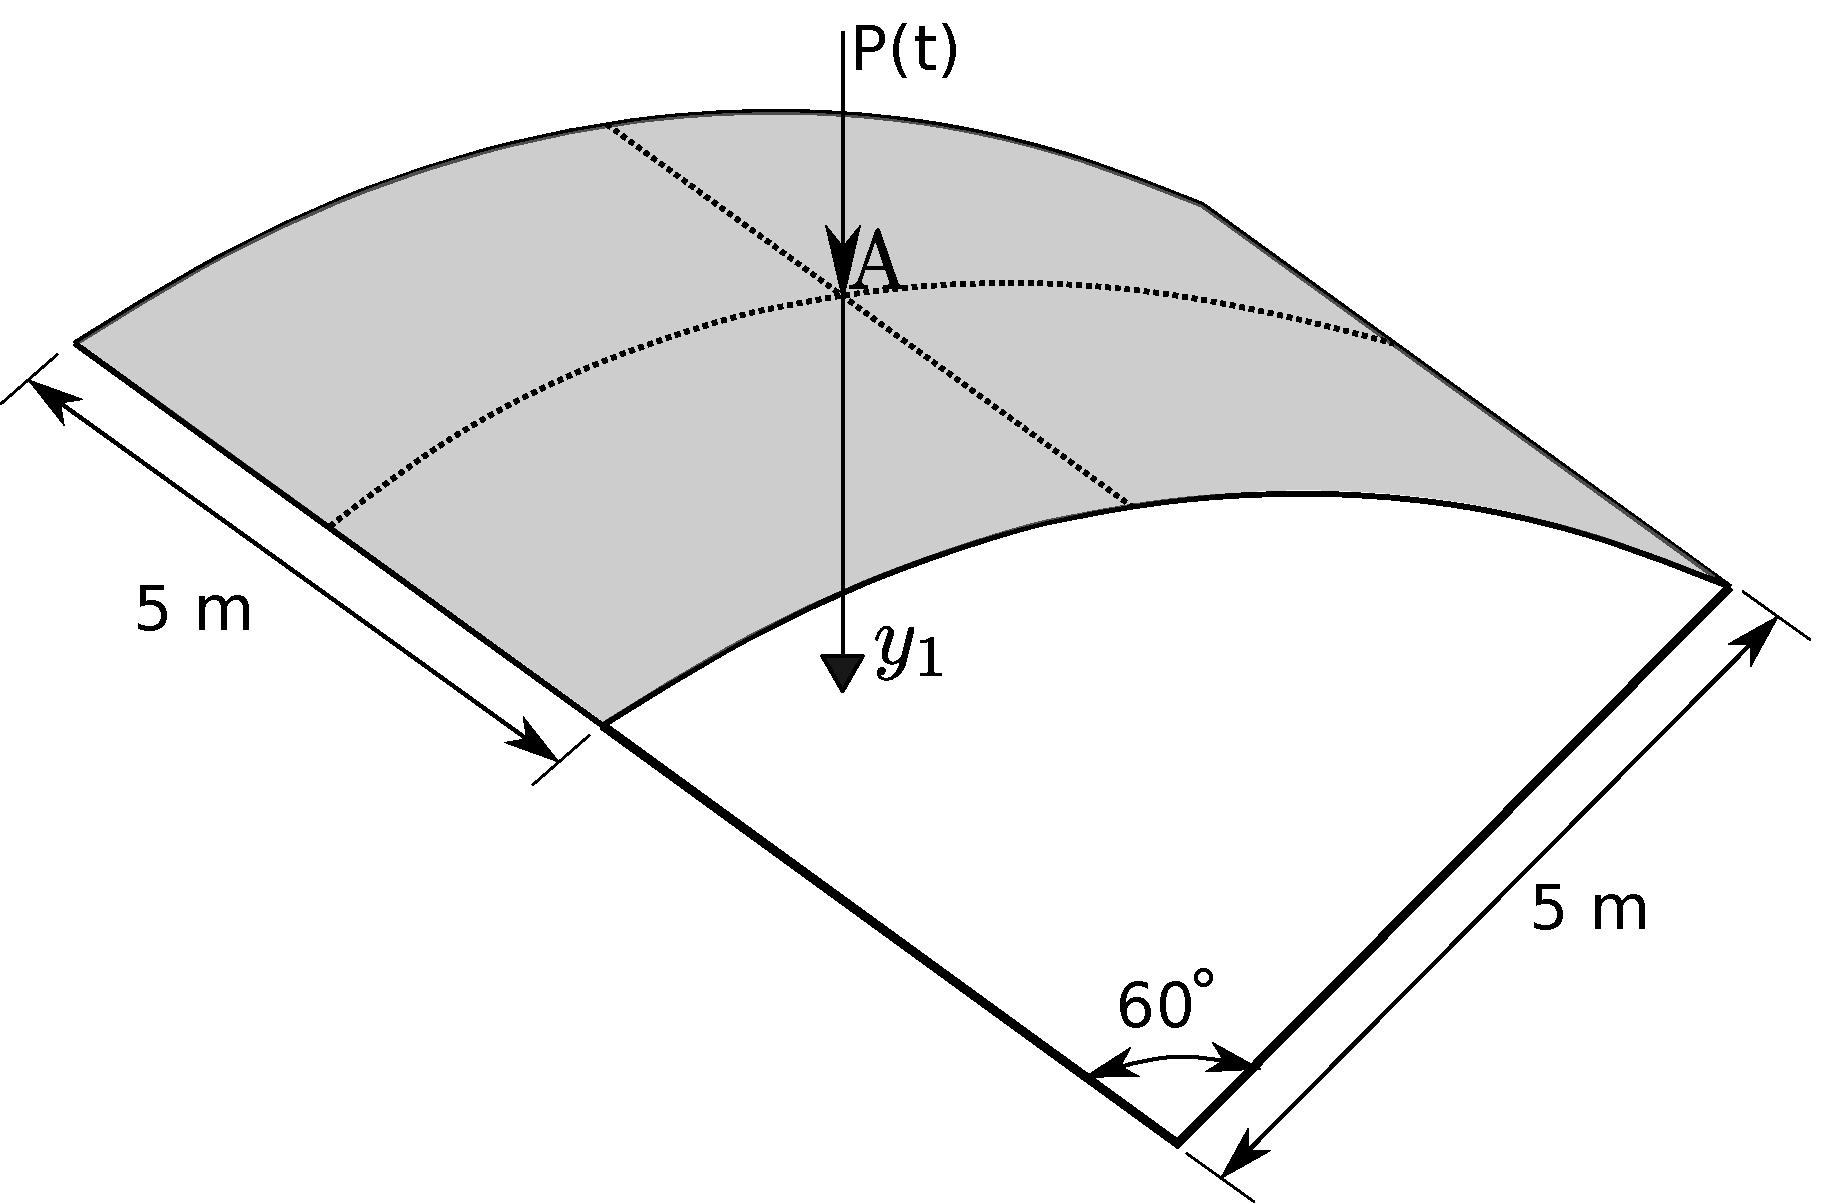
\includegraphics[scale=0.23, trim=0cm 0cm 0cm 0cm, clip=true]{Imagens/Cap4/casca_geometria.pdf}} 
	\subfloat[\label{fig:casca_malha} Malha ]{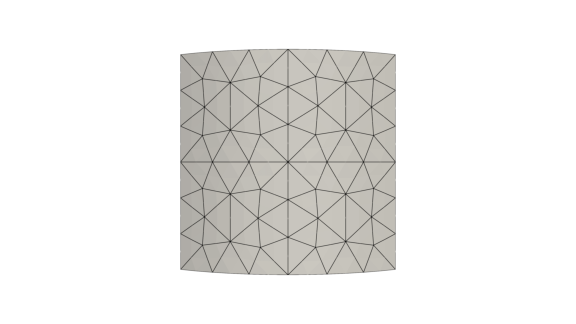
\includegraphics[scale=1.1,trim=2cm 0.5cm 2cm 0.5cm, clip=true]{Imagens/Cap4/casca_malha.pdf}}
	\label{fig:Casca}
	\legend{Fonte: Elaborada pela autora}
\end{figure}

Os contornos esquerdo e direito da chapa são considerados simplesmente apoiados. O carregamento aplicado ao ponto central (ponto A) $P(t)$ é aplicado linearmente no intervalo $t=0s$ até $t=0,2s$, com $P(0)=0kN$ e $P(2s) = 200000kN$, e então mantido constante. As características físicas do material utilizado são: $\elasticModulus = 200GPa$, $\poisonsRatio = 0,25$ e $\rho = 10000 kg/m^3$ e o passo de tempo adotado na simulação é $\Delta_{t} = 0,001s$.

O deslocamento vertical do nó central da casca obtido nesse trabalho pode ser visualizado na \autoref{fig:casca_deslocamentoA}, enquanto que, para o autor de referência na \autoref{fig:casca_deslocamento_ref}. O resultado obtido está de acordo com os resultados de \citeonline{ArgyrisPM:2003}. Os campos de deslocamentos para os instantes $t = 140ms$, $t = 165ms$, $t = 174ms$ e $t = 177ms$ são apresentados na Figura \ref{fig:casca_campos_deslocamentos}.

\begin{figure}[!htbp]
	\caption{Casca: Deslocamento vertical nó central A}
	\centering
	{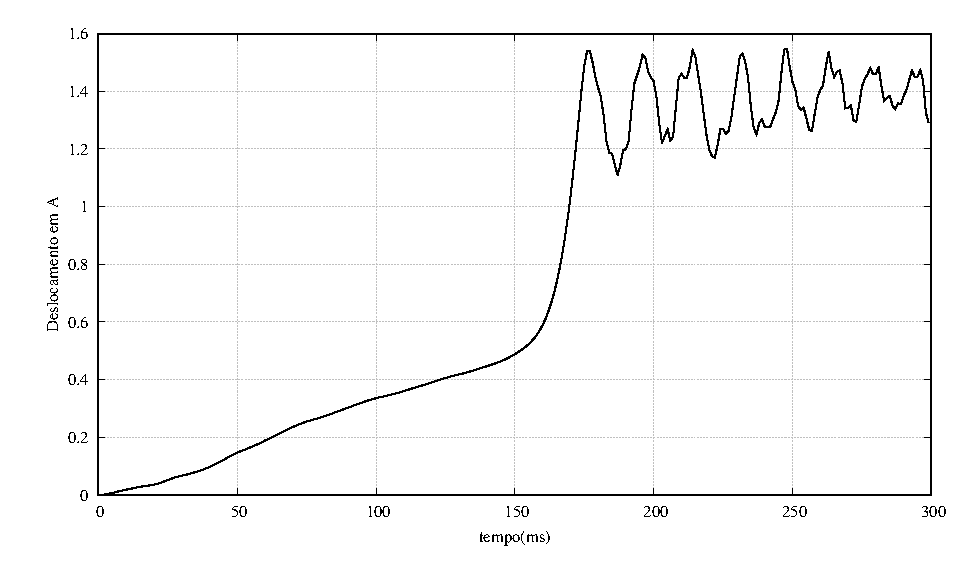
\includegraphics[scale=.6, trim=0cm 0cm 0cm 0cm, clip=true]{Imagens/Cap4/casca_deslocamentoA.eps}}
	\label{fig:casca_deslocamentoA}
	\legend{Fonte: Elaborada pela autora}
\end{figure}

\begin{figure}[!htbp]
	\caption{Casca: Deslocamento vertical nó central A - referência}
	\centering
	{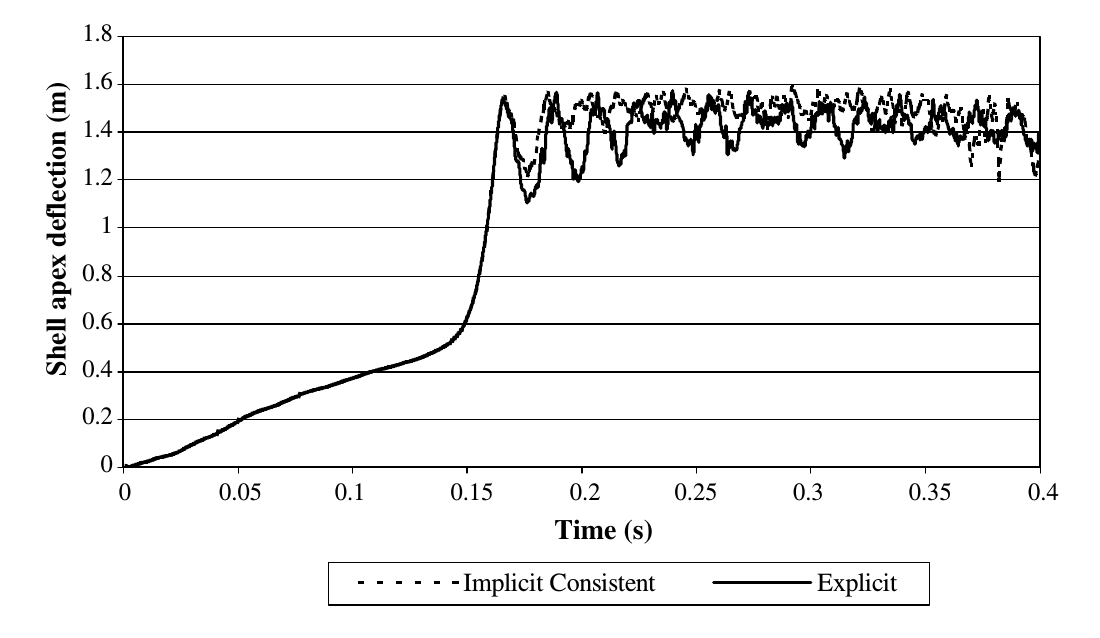
\includegraphics[scale=0.25,trim=0cm 0cm 0cm 0cm, clip=true]{Imagens/Cap4/casca_deslocamento_referencia.png}}
	\legend{Fonte: \citeonline{ArgyrisPM:2003}}
	\label{fig:casca_deslocamento_ref}
\end{figure}

\begin{figure}[!htbp]
	\caption{Casca: Campos de deslocamentos}
	\centering
	\subfloat[\label{fig:casca_140ms} $t = 140ms$.]{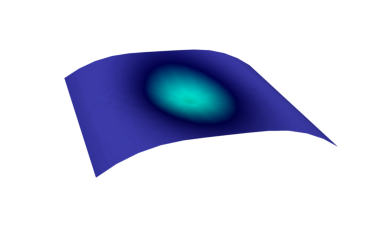
\includegraphics[scale=1.3, trim=0.8cm 0.4cm 0.8cm 0.8cm, clip=true]{Imagens/Cap4/casca_140ms.pdf}}
	\subfloat[\label{fig:casca_165ms} $t = 165ms$.]{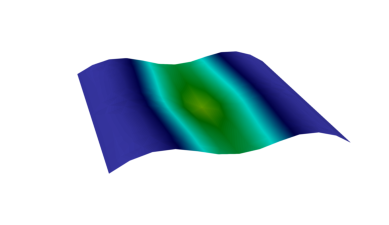
\includegraphics[scale=1.3, trim=0.8cm 0.4cm 0.8cm 0.8cm, clip=true]{Imagens/Cap4/casca_165ms.pdf}} \\
	\subfloat[\label{fig:casca_174ms} $t = 174ms$.]{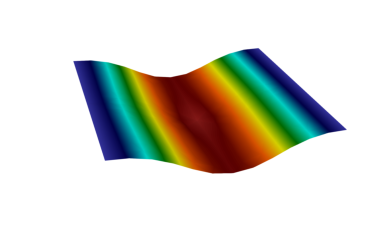
\includegraphics[scale=1.3, trim=0.7cm 0.4cm 0.7cm 0.8cm, clip=true]{Imagens/Cap4/casca_174ms.pdf}}
	\subfloat[\label{fig:casca_177ms} $t = 177ms$.]{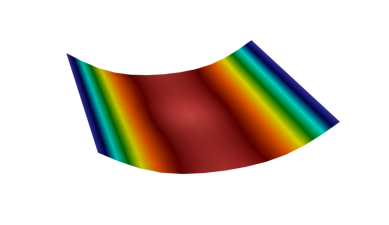
\includegraphics[scale=1.3, trim=0.7cm 0.4cm 0.7cm 0.8cm, clip=true]{Imagens/Cap4/casca_177ms.pdf}} \\
	{\includegraphics[scale=0.015,trim=0cm 20.0cm 0cm 0cm, clip=true]{Imagens/Cap4/casca_legenda.pdf}}
	\label{fig:casca_campos_deslocamentos}
	\legend{Fonte: Elaborada pela autora}
\end{figure}